\chapter{Representation of vortex variability in climate models}
\label{cha:models}


\section{Introduction}


Over the past decade an increasing number of climate models have included a
well-resolved stratosphere, with model lids above the stratopause. For example,
the fifth Coupled Model Intercomparison Project (CMIP5) \citep{Taylor2012}
includes 15 models with an uppermost level above the stratopause, whereas the
previous intercomparison project, CMIP3, includes only 5
\citep{Cordero2006}. The CMIP5 model simulations are significant in that they
are motivated by, and evaluated in the the Intergovernmental Panel on Climate
Change (IPCC) Fifth Assessment Report (AR5) \citep{Stocker2013}. This change in
model stratospheric resolution has been largely motivated by an increased
understanding of the stratosphere's influence on tropospheric climate (discussed
in \citet{Gerber2012} and Chapters \ref{cha:introduction} and
\ref{cha:moments}).

The effect of this greater stratospheric resolution was studied by
\citet{Charlton-Perez2013}, who compared stratospheric variability between
high-top and low-top models within the CMIP5 ensemble (they defined ``high-top''
as a model lid above 1~hPa, and ``low-top'' below). They found that the low-top
models have a weaker and less realistic representation of daily to interannual
polar stratospheric variability than high-top models. They attribute this to the
fact that the low-top models simulate fewer SSW events than high-top. This is
combined with a slightly weaker tropospheric NAM response in the two months
following SSW events in the low-top compared to high-top models.

These results are supported by similar studies which compare high and low-top
versions of the same model. \citet{Cagnazzo2009} found that a high-top model
gave a more realistic representation of the influence of ENSO on the NH
extratropical stratosphere. Similarly, \citet{Hardiman2012a} showed the
influence of the QBO on the extratropics as well as decadal trends in the NAO
were more realistically simulated by the high-top than the low-top model. These
differences have again been linked to the different simulation of SSW events in
high- and low-top models \citep{Sassi2010}. 

Other studies have compared simulations of climate change with high- and low-top
models. \citet{Huebener2007} linked a increased weakening of the stratospheric
polar vortex in high-top similations to a more southward shift of the NH winter
storm track, which in turn affects trends in North Atlantic temperatures and
precipitation. \citet{Manzini2014} investigated climate change simulations of
high- and low-top models in the CMIP5 ensemble. They found that the inter-model
spread in the simulation of changes of stratospheric polar vortex winds accounts
for a significant fraction of the inter-model spread of trends in the surface
NAM under climate change. Interestingly, \citet{Manzini2014} also show that
global surface temperature trends under climate change (and so climate
sensitivity) are larger for high-top compared to low-top models. However, when
comparing pairs of high- and low-top versions of the same (or similar) models,
little in climate sensistivity difference is detected, and they conclude that
this difference is unlikely to have a physical basis.

Despite these findings about the differences between high- and low-top models,
it is important to note that a model lid above the stratopause is not a
sufficient condition for the accurate representation of stratospheric processes
or stratosphere-troposphere coupling. Indeed, \citet{Charlton-Perez2013} found
that the frequency of SSWs in high-top CMIP5 models varies widely, from about
2.5 to 8 events per decade. 

In this chapter we apply the methods developed in Chapter \ref{cha:moments} to
evaluate the representation of stratospheric polar vortex variability in
contemporary climate models. We wish to perform as much as possible, a
like-for-like comparison, and so select only models with a lid height above the
stratopause. In doing this we extend the work of \citet{Charlton-Perez2013} to
consider the two-dimensional structure of the polar vortex, including split and
displaced vortex events. We also consider the influence of these events on the
troposphere in each model. 

There are three main objectives to this investigation. First, we wish to
evaluate the current state of model's representation of the stratospheric polar
vortex and stratosphere-troposphere coupling, including whether there are any
consistent biases among models. Second, we aim to determine if there is a
relationship between model parameters (such as horizontal and vertical
resolution) and biases in their representation of vortex variability. This may
motivate future model improvements to reduce these biases. Third, we investigate
whether the increased sample size of the CMIP5 ensemble can be used to better
understand the mechanism behind the different tropospheric response to split and
displaced vortex events, which was described in Chapter \ref{cha:moments}. 

\subsection{CMIP5 model simulations}

For this analysis, only climate models with a lid height above the stratopause
are selected from the CMIP5 ensemble. In total, 13 such models were available
from 8 different modelling centres, although another two (CESM1-WACCM and
MIROC-ESM) are listed in the CMIP5 ensemble, appropriate data was not found to
be available for these models in the CMIP5 archive
(http://pcmdi3.llnl.gov/esgcet/home.htm). These models are listed in Table
\ref{tab:models}. It can be seen that 12 of the 13 models have an uppermost
level which is in the upper mesosphere (70-80~km), but CanESM2 has a
significantly lower lid which is very close to the stratopause.

Historical simulations have been used throughout this analysis. These include
observed climate forcings, such as from greenhouse gasses, ozone depletion,
land-use change, tropospheric and stratospheric aerosols and solar
variability. The simulation period considered is limited to 1958-2005, so that
it coincides with the ERA-40/ERA-Interim reanalysis period (CMIP5 historical
simulations end at 2005), therefore allowing for a more direct comparison with
observations. In order to achieve the largest possible ensemble size, all
available ensemble members have been used for each model, which leads to a
differing number of years entering the ensemble from different models.

\begin{table}[htbp]
\small
\centering
\begin{tabular}{lcccccc} \hline
Model          & Ensemble size & Lid/ km & Levels & dh/km & d$z_{1}$/km & d$z_{2}$/km \\ \hline
CanESM2        & 5 & 48.1    & 35     & 268          & 1.48         & 2.30          \\
CMCC-CESM      & 1 & 80.6    & 39     & 536          & 1.49         & 1.89          \\
CMCC-CMS       & 1 & 80.6    & 95     & 268          & 0.65         & 0.68          \\
GFDL-CM3       & 5 & 76.3    & 48     & 191          & 1.32         & 1.75           \\
HadGEM2-CC     & 3 & 84.1    & 60     & 144          & 0.82         & 1.18          \\
IPSL-CM5A-LR   & 5 & 70.4    & 39     & 254          & 1.21         & 1.75          \\
IPSL-CM5A-MR   & 3 & 70.4    & 39     & 169          & 1.21         & 1.75          \\
IPSL-CM5B-LR   & 1 & 70.4    & 39     & 254          & 1.21         & 1.75          \\
MIROC-ESM-CHEM & 1 & 87.8    & 80     & 399          & 0.77         & 0.73          \\
MPI-ESM-LR     & 3 & 80.6    & 47     & 268          & 0.87         & 1.70            \\
MPI-ESM-MR     & 3 & 80.6    & 95     & 268          & 0.65         & 0.68          \\
MRI-CGCM3      & 1 & 80.6    & 48     & 107          & 0.88         & 1.87          \\
MRI-ESM1       & 1 & 80.6    & 48     & 107          & 0.88         & 1.87 \\ \hline 
\end{tabular}
\caption[CMIP5 model parameters.]{Parameters of the CMIP5 models studied in this
  chapter. Where the model lid is defined in terms of a pressure, its height was
  estimated using $z=-H\mathrm{ln}(p/p_{0})$ with $H=7$~km and
  $p_{0}=1000$~hPa. Horizontal resolution, d$h$, is estimated at 45$^{\circ}$N
  and vertical resolution is shown averaged over two regions; 5-15~km (d$z_{1}$)
  and 15-30~km (d$z_{2}$).} 
\label{tab:models}
\end{table}




\section{Vortex mean state and variability}
\subsection{Moment diagnostics}

\begin{figure}[htbp]
 \centering
 \noindent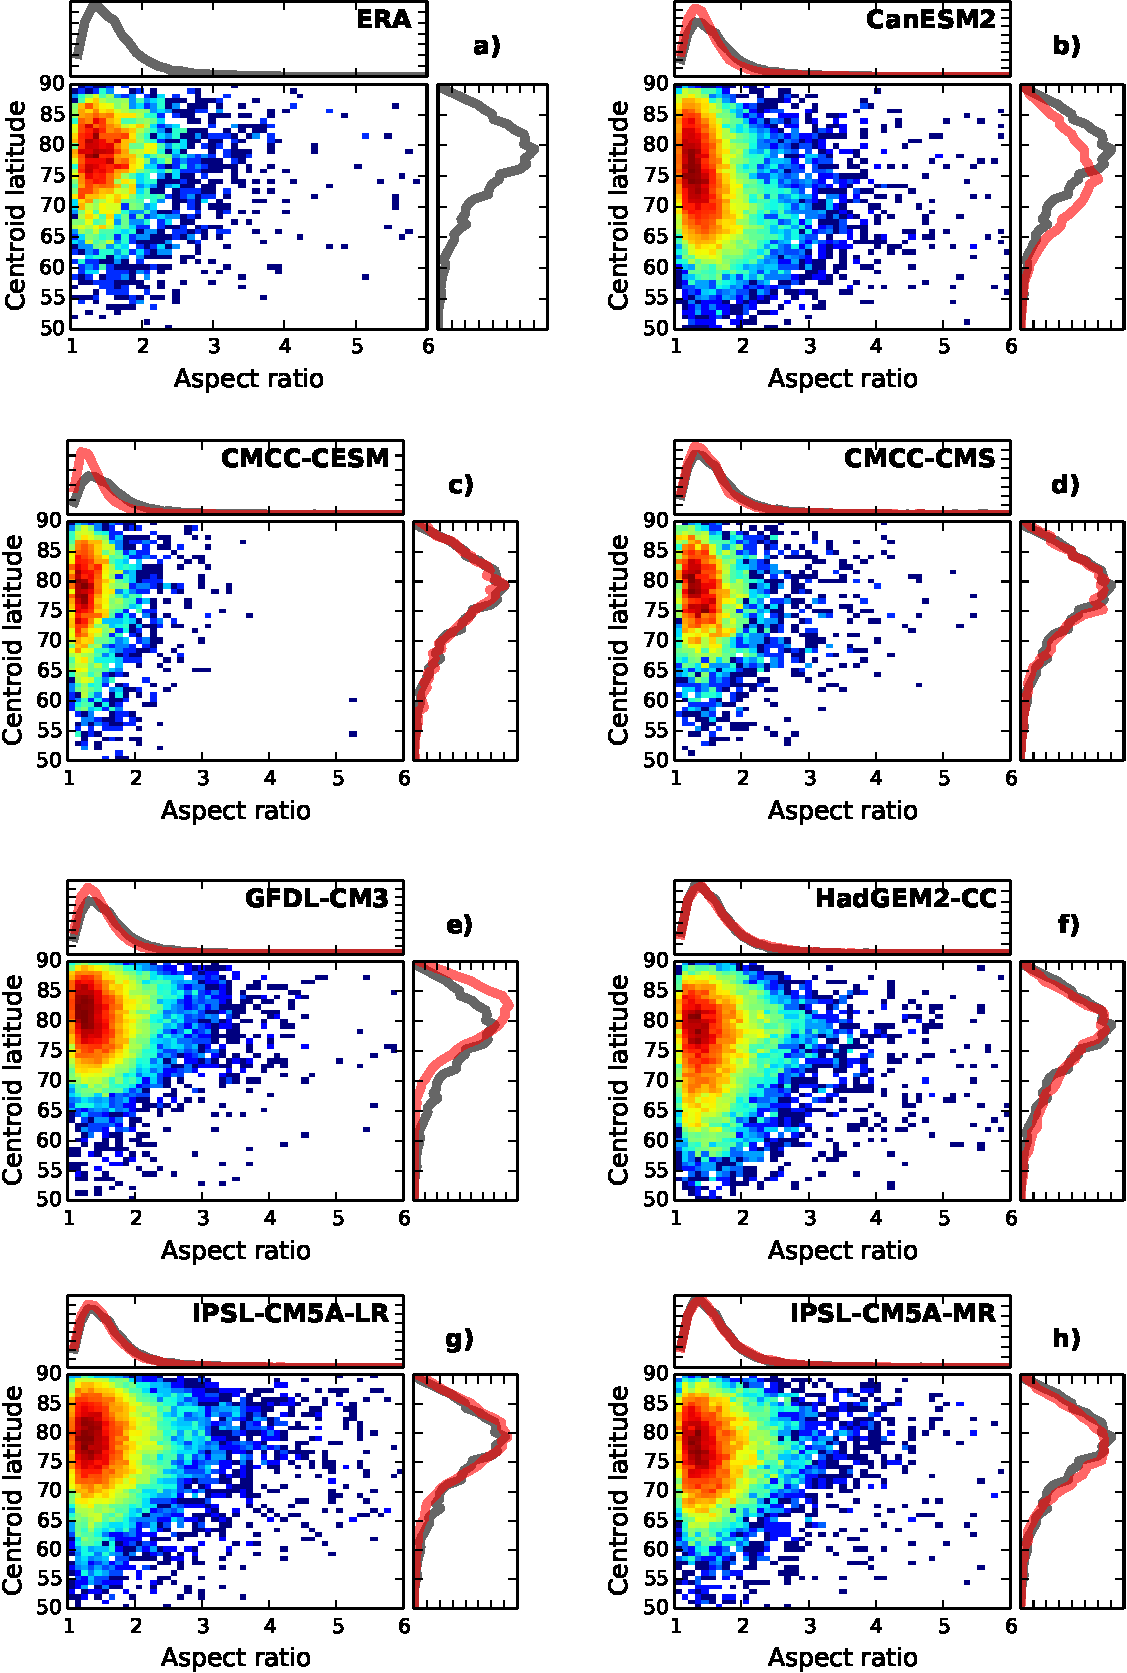
\includegraphics[width=\textwidth]{figures/chapter-models/moments_stats1.pdf}
 \caption[Distributions of moment diagnostics for the CMIP5
 models.]{Distributions of centroid latitude and aspect ratio for the ERA (grey
   lines) (a) and the CMIP5 models (red lines). Joint distributions are shown
   with a logarithmic scale such that red squares represent the densest
   regions.}
 \label{fig:cmip5_moments_stats}
\end{figure}

\begin{figure}[htbp]
 \ContinuedFloat
 \centering
 \noindent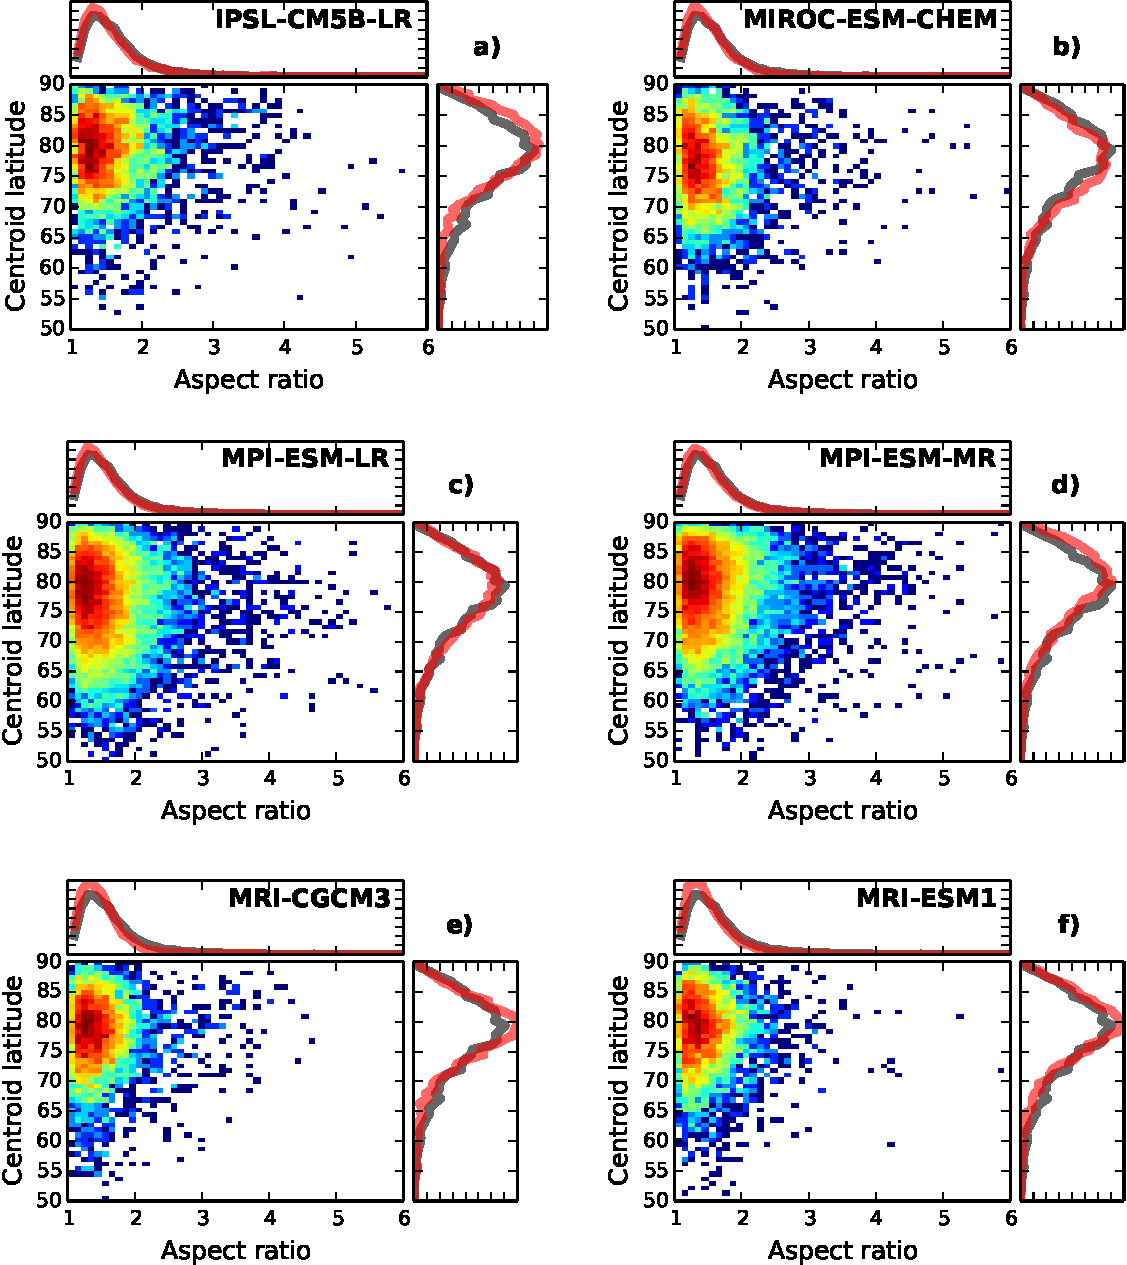
\includegraphics[width=\textwidth]{figures/chapter-models/moments_stats2.pdf}
 \caption[]{(Continued)}
\end{figure}


The centroid latitude and aspect ratio moment diagnostics are calculated for
each of the CMIP5 models over DJFM from the 10~hPa geopotential height field,
using the method described in Section \ref{sec:vort-geom-calc}. For each model
the value of the DJFM mean geopotential height at 60$^{\circ}$N and 10~hPa is
used to define the appropriate contour for the calculation of the moment
diagnostics. This accounts for biases in the mean geopotential height between
different models.

The resulting joint distributions of daily centroid latitude and aspect ratio
from each of the models are shown in Figure \ref{fig:cmip5_moments_stats}, along
with that from the ERA-40/ERA-Interim reanalysis (hereafter ERA) calculated in
Chapter \ref{cha:moments}. For each model the joint distribution histogram is
plotted with a logarithmic colour scale which is normalised according to the
number of days entering each box. As discussed in Chapter \ref{cha:moments}, it
can be seen that the joint distribution for ERA has an approximately triangular
distribution with high aspect ratio/poleward centroid latitude, and low aspect
ratio/equatorward centroid latitude being relatively more common than
high aspect ratio/equatorward centroid latitude. This shape of distribution is
well replicated by most of the models, although CanESM2 has a significantly
different shape, with the high aspect ratio/equatorward centroid latitude being
more common. 

No clear consistent biases among models emerge from this analysis. CanESM2 has a
modal centroid latitude which is about $5^{\circ}$ too far equatorward compared
to reanalysis. Contrastingly, GFDL-CM3 has a modal centroid latitude about
$2.5^{\circ}$ more poleward than observed. CMCC-CESM displays a clear bias in
the aspect ratio, with a distribution much less skewed towards high values than
in reanalysis.

The winter seasonal cycle of aspect ratio and centroid a latitude in the CMIP5
models is shown in Figure \ref{fig:cmip5_moments_stats_seas}. For the mean
aspect ratio and centroid latitude, the majority of models agree well with
reanalysis. CMCC-CESM has a consistently too low mean aspect ratio, while
GFDL-CM3 has a consistently too poleward mean centroid latitude, indicating that
these biases are not strongly seasonally dependent. On the other hand, the large
equatorward bias in the CanESM2 mean centroid latitude is much larger in
December and early January than later in winter. The 95th percentile of aspect
ratio is lower than reanalysis for the majority of models throughout the season,
indicating that models have, on average, too little variability in aspect ratio
 
\begin{figure}
 \centering
 \noindent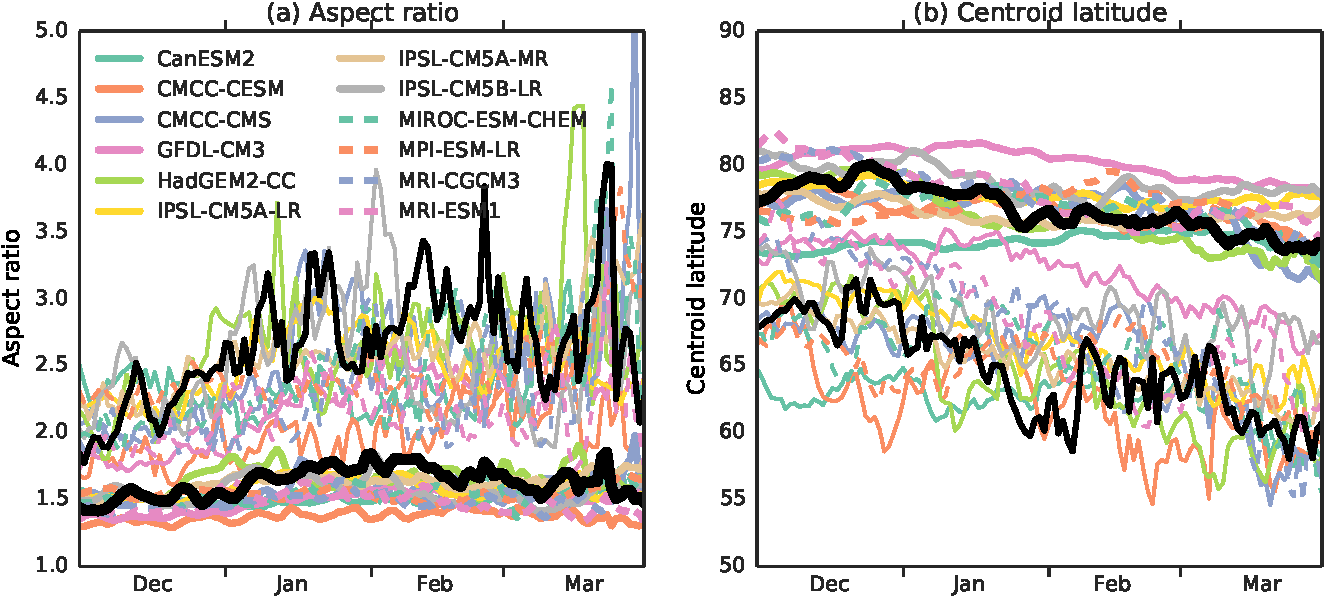
\includegraphics[width=\textwidth]{figures/chapter-models/moments_seasonal_stats.pdf}
 \caption[Seasonal cycle of moment diagnostics in the CMIP5 models]{Seasonal
   cycle of aspect ratio and centroid latitude in ERA (black) and the CMIP5
   models (colours). Thick lines represent the mean and thin lines the 95th or
   5th percentile for aspect ratio and centroid latitude respectively.}
 \label{fig:cmip5_moments_stats_seas}
\end{figure}


\subsection{Displaced and split vortex events}

Displaced and split vortex events are identified within the CMIP5 ensemble using
the threshold-based method described in Section \ref{sec:event-definition}. The
same thresholds as used for ERA (66$^{\circ}$N for centroid latitude and 2.4 for
aspect ratio) are used for the models in order to identify, as much as possible,
geometrically equivalent events. The same persistence of 7 days was also used.
The frequency of displaced and split vortex events for each model is shown in
Figure \ref{fig:cmip5_events_bar_stacked}.

\begin{figure}[htbp]
 \centering
 \noindent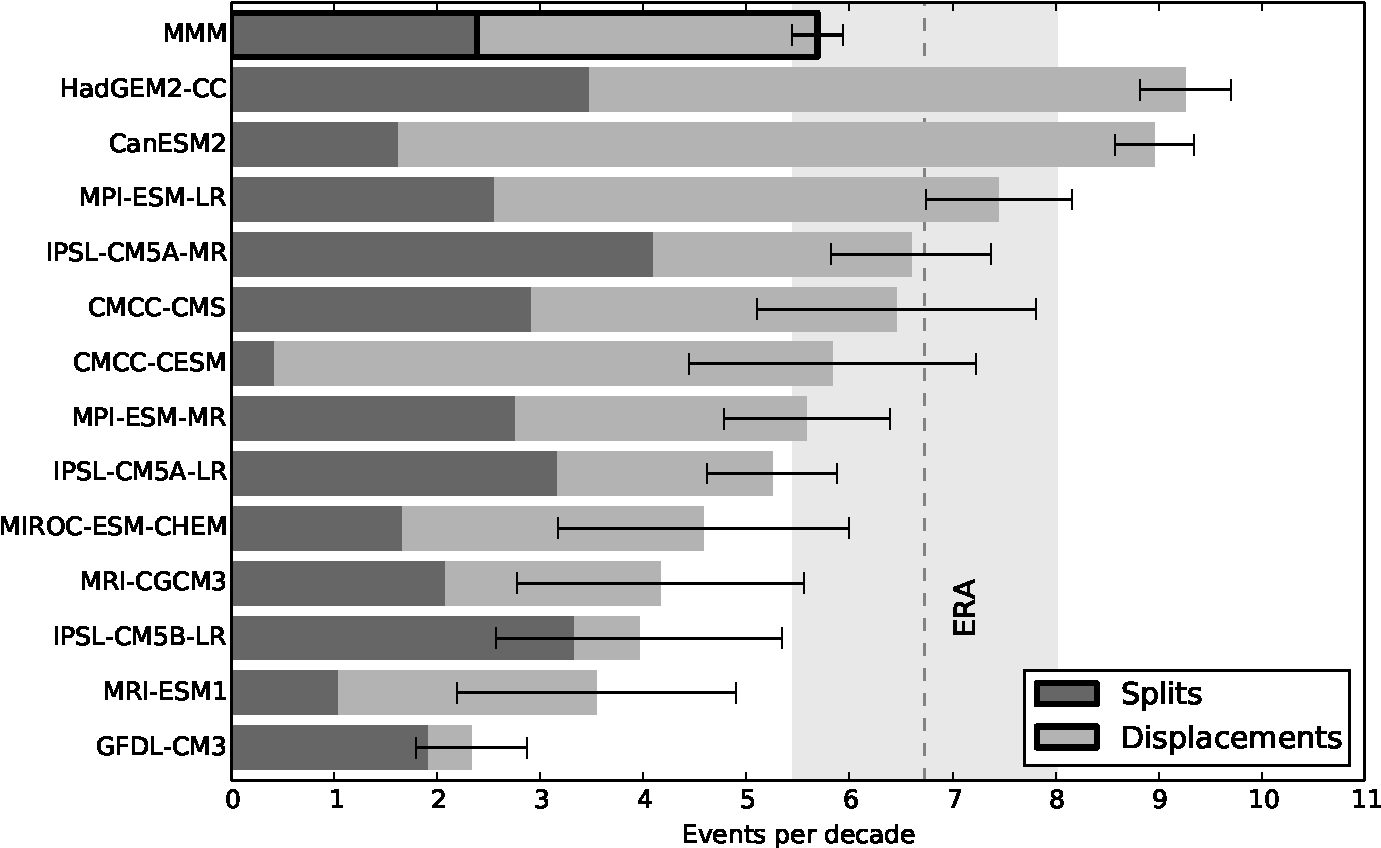
\includegraphics[width=\textwidth]{figures/chapter-models/events_bar_stacked.pdf}
 \caption[Frequency of split and displaced vortex events in the CMIP5
 models]{Frequency of split and displaced vortex events in the CMIP5 models,
   ERA, and the multi-model mean (MMM). Error bars are for the frequency of all
   events, and represent one $\sigma$ range, assuming a binomial distribution of
   events. The grey shaded region represents the one $\sigma$ range for ERA,
   along with the mean (dashed line.) }
 \label{fig:cmip5_events_bar_stacked}
\end{figure}

% Look at Charlton-Perez 2013 to see which models have lowest frequency

The total frequency of displaced and split vortex events for each of the CMIP5
models agrees well with the equivalent SSW frequency calculated by
\citet{Charlton-Perez2013}, who identified events based on the reversal of
zonal-mean zonal wind at 60$^{\circ}$N and 10~hPa. They also found that
HadGEM2-CC to have the highest frequency of events within the CMIP5 ensemble,
while ?? and ?? were the models with the lowest freqency of SSWs in their study
(they did not analyze GFDL-CM3, which we find to have the lowest frequency of
events). This similarlity between \citet{Charlton-Perez2013} and the present
study indicates that the close relationship between moment diagnostics-defined
events and SSWs defined by zonal-mean zonal wind, as described in Chapter
\ref{cha:moments}, also holds for climate models (although this is not
explicitly shown here).

It can be seen in Figure \ref{fig:cmip5_events_bar_stacked} that the ratio of
frequencies of displaced to split vortex events varies significantly between
models. For instance CanESM2 and CMCC-CESM simulate almost entirely displaced
vortex events, while IPSL-CM5B-LR and GFDL-CM3 simulate almost entirely split
vortex events. In the multi-model mean (MMM) these biases largely cancel, to
give a approximately equal ratio of displaced to split vortex events, which is
in agreement with reanalysis.  

The seasonal distribution of these displaced and split vortex events is
illustrated in Figure \ref{fig:cmip5_events_seasonal}. Some models replicate the
observed distribution, with split vortex events being more likely in early
winter, and displaced vortex events in late winter; these models are CMCC-CMS,
HadGEM2-CC and IPSL-CM5A-LR. Other models, however, have a very different
distribution. % More description here

\begin{figure}
 \centering
 \noindent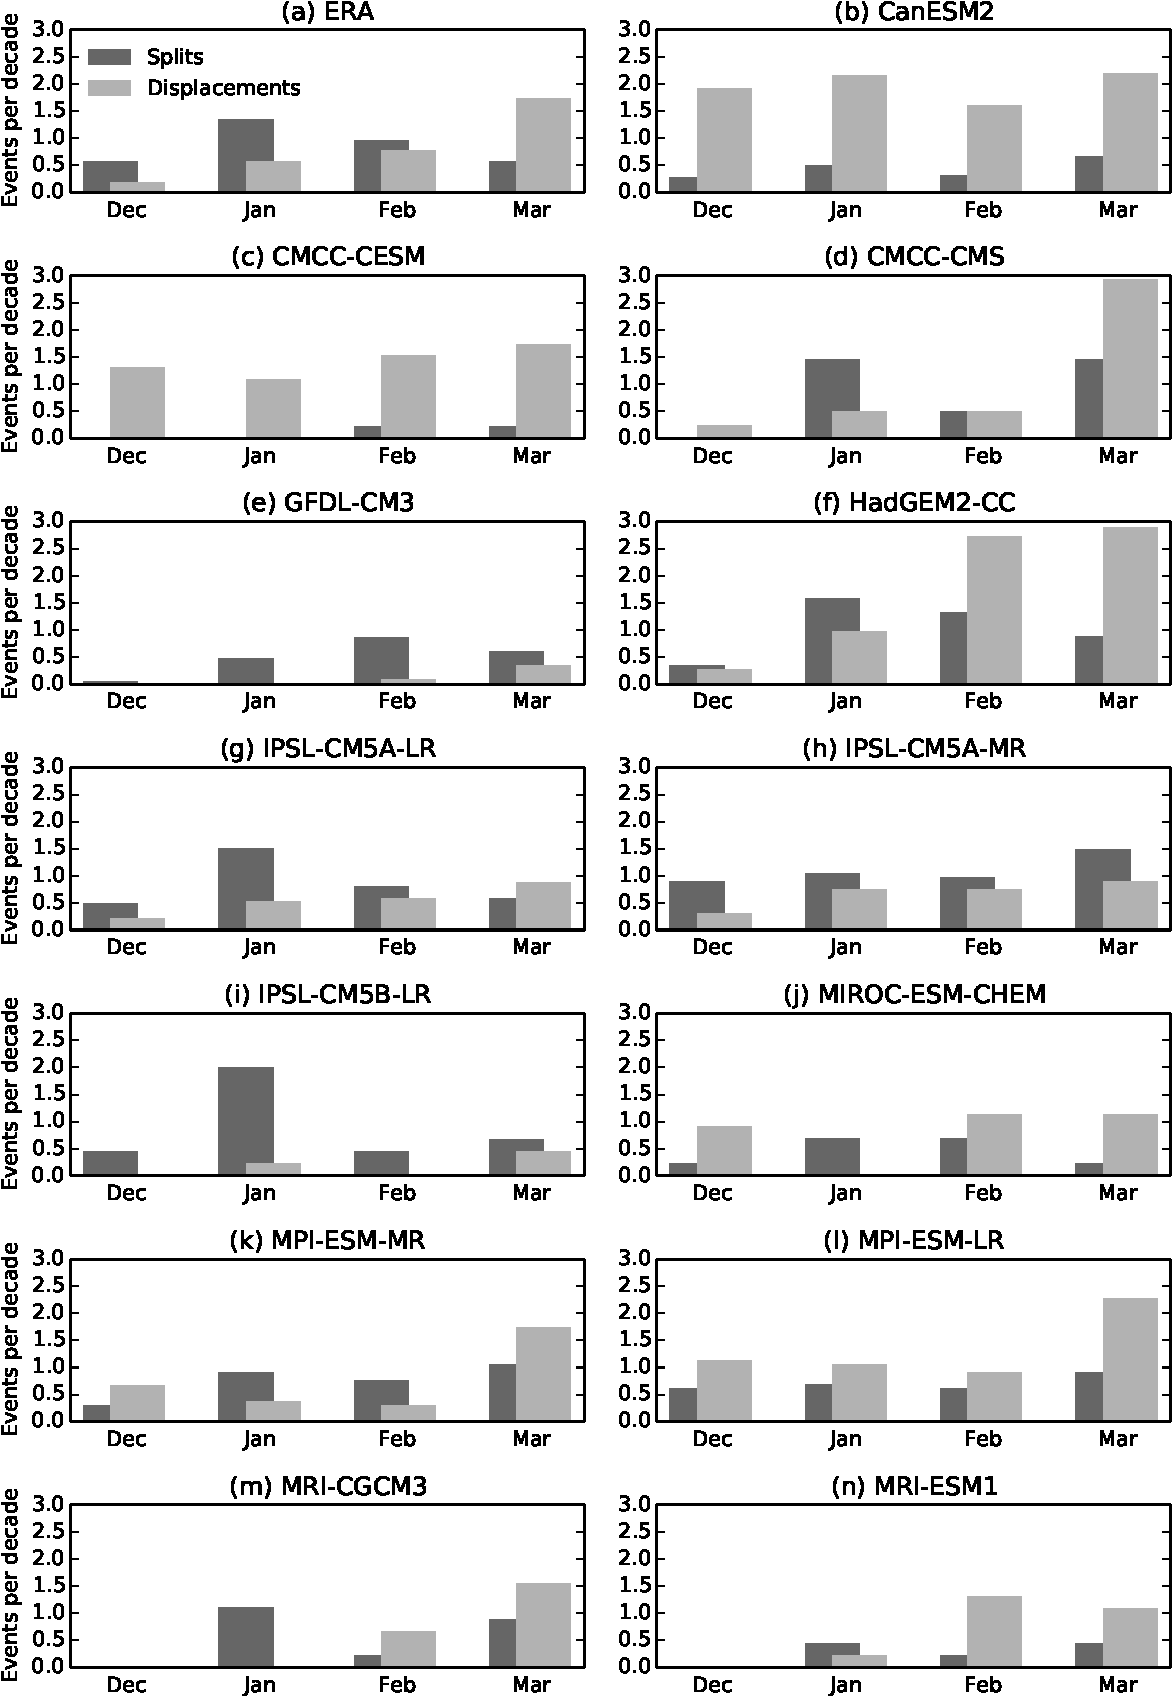
\includegraphics[width=\textwidth]{figures/chapter-models/events_seasonal.pdf}
 \caption[Seasonal distribution of splits and displacements in the CMIP5
 models]{Seasonal distribution of the occurrence of split and displaced vortex
   events in ERA (a) and the CMIP5 models.}
 \label{fig:cmip5_events_seasonal}
\end{figure}

It is noteworthy that the model with the largest equatorward bias in the mean
centroid latitude, CanESM2, also has the highest frequency of displaced vortex
events. Indeed, the relationship between model mean moment diagnostics and
frequency of displaced and split vortex events is illustrated in Figure
\ref{fig:cmip5_moments_scatter}. This indicates that there is a strong
correlation between model mean values and frequency of events. The correlations
shown indicate that mean biases in aspect ratio account for 85\% of the
inter-model spread in the frequency of split vortex events, while mean biases in
centroid latitude account for 77\% of the spread in frequency of displaced
vortex events. This indicates that the largest improvements in model simulations
of the frequency of displaced and split vortex events can come about through a
more realistic mean climatology of the vortex, rather than changes in the model
variability.

% REPEAT for mode??
\begin{figure}
 \centering
 \noindent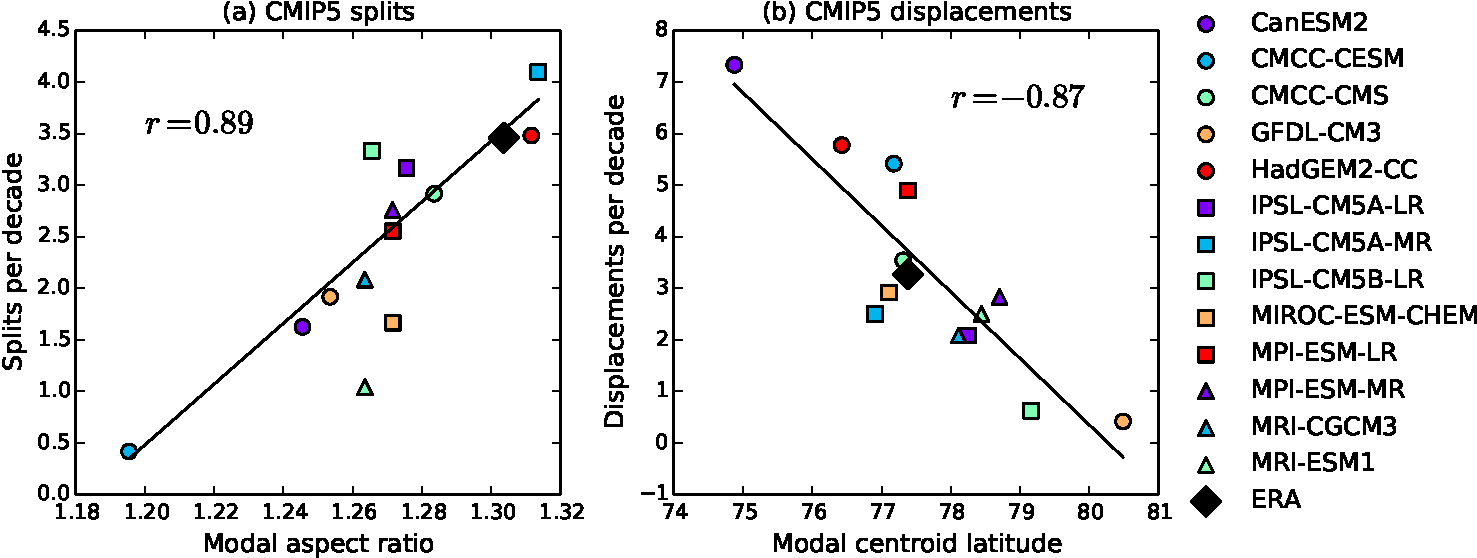
\includegraphics[width=\textwidth]{figures/chapter-models/CMIP5_moments_scatter.pdf}
 \caption[Comparison of moment diagnostics and frequency of split and displaced
 vortex events.]{Comparison of the DJFM mean aspect ratio with frequency of
   split vortex events (a) and DJFM mean centroid latitude with frequency of
   displaced vortex events (b) in the CMIP5 ensemble and ERA. A linear best fit
   and the correlation coefficients for all the models are also shown.}
 \label{fig:cmip5_moments_scatter}
\end{figure}

The structure of the stratospheric polar vortex during split and displaced
vortex events in the CMIP5 ensemble is shown in Figure
\ref{fig:10hPa_GPH_comp}. This shows composites of 10~hPa geoopotential height
at the onset date of the events for each model. The absolute values of the
contours are different for each model due to differences in climatology,
although the spacing between contours remains constant. It can be seen that the
majority of models accurately reproduce splitting events occuring along the
$90^{\circ}$W-$90^{\circ}$E line, and displacement events with a vortex shifted
towards Scandinavia and Siberia. CanESM2 is an exception to this, with split
vortex events which are centred quite far from the pole. The IPSL-CM5B-LR model
also has a very different appearance of 


\begin{figure}
 \centering
 \noindent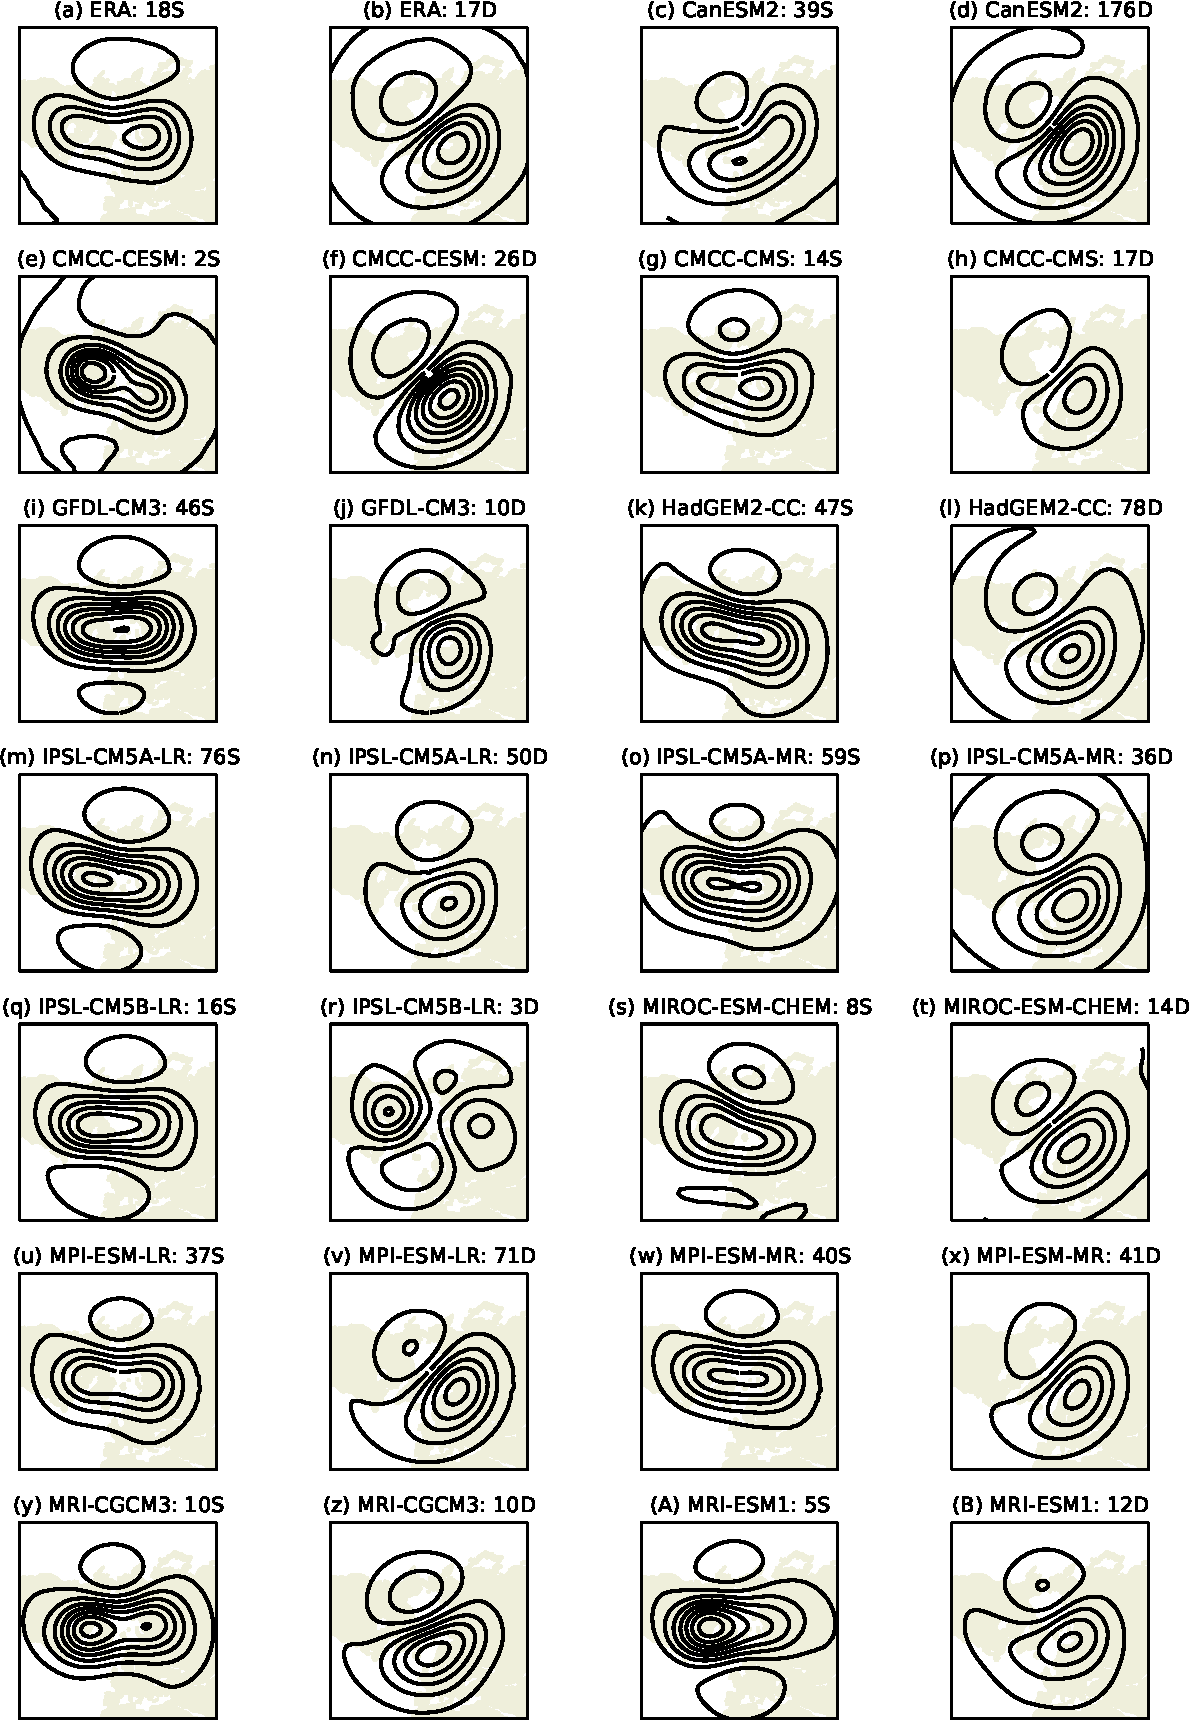
\includegraphics[width=\textwidth]{figures/chapter-models/10hPa_GPH_composites.pdf}
 \caption[Composites of 10~hPa $Z$ at the onset date split and displaced vortex
 events in the CMIP5 models.]{Composites of 10~hPa $Z$ at the onset date of
   split (S) and displaced (D) vortex events in ERA (a,b) and the CMIP5
   models. The number of events entering the composite and their type are
   shown in the title of each plot. The contour interval is 0.3~km.}
 \label{fig:10hPa_GPH_comp}
\end{figure}




\section{Stratosphere-troposphere coupling}

\begin{figure}
 \centering
 \noindent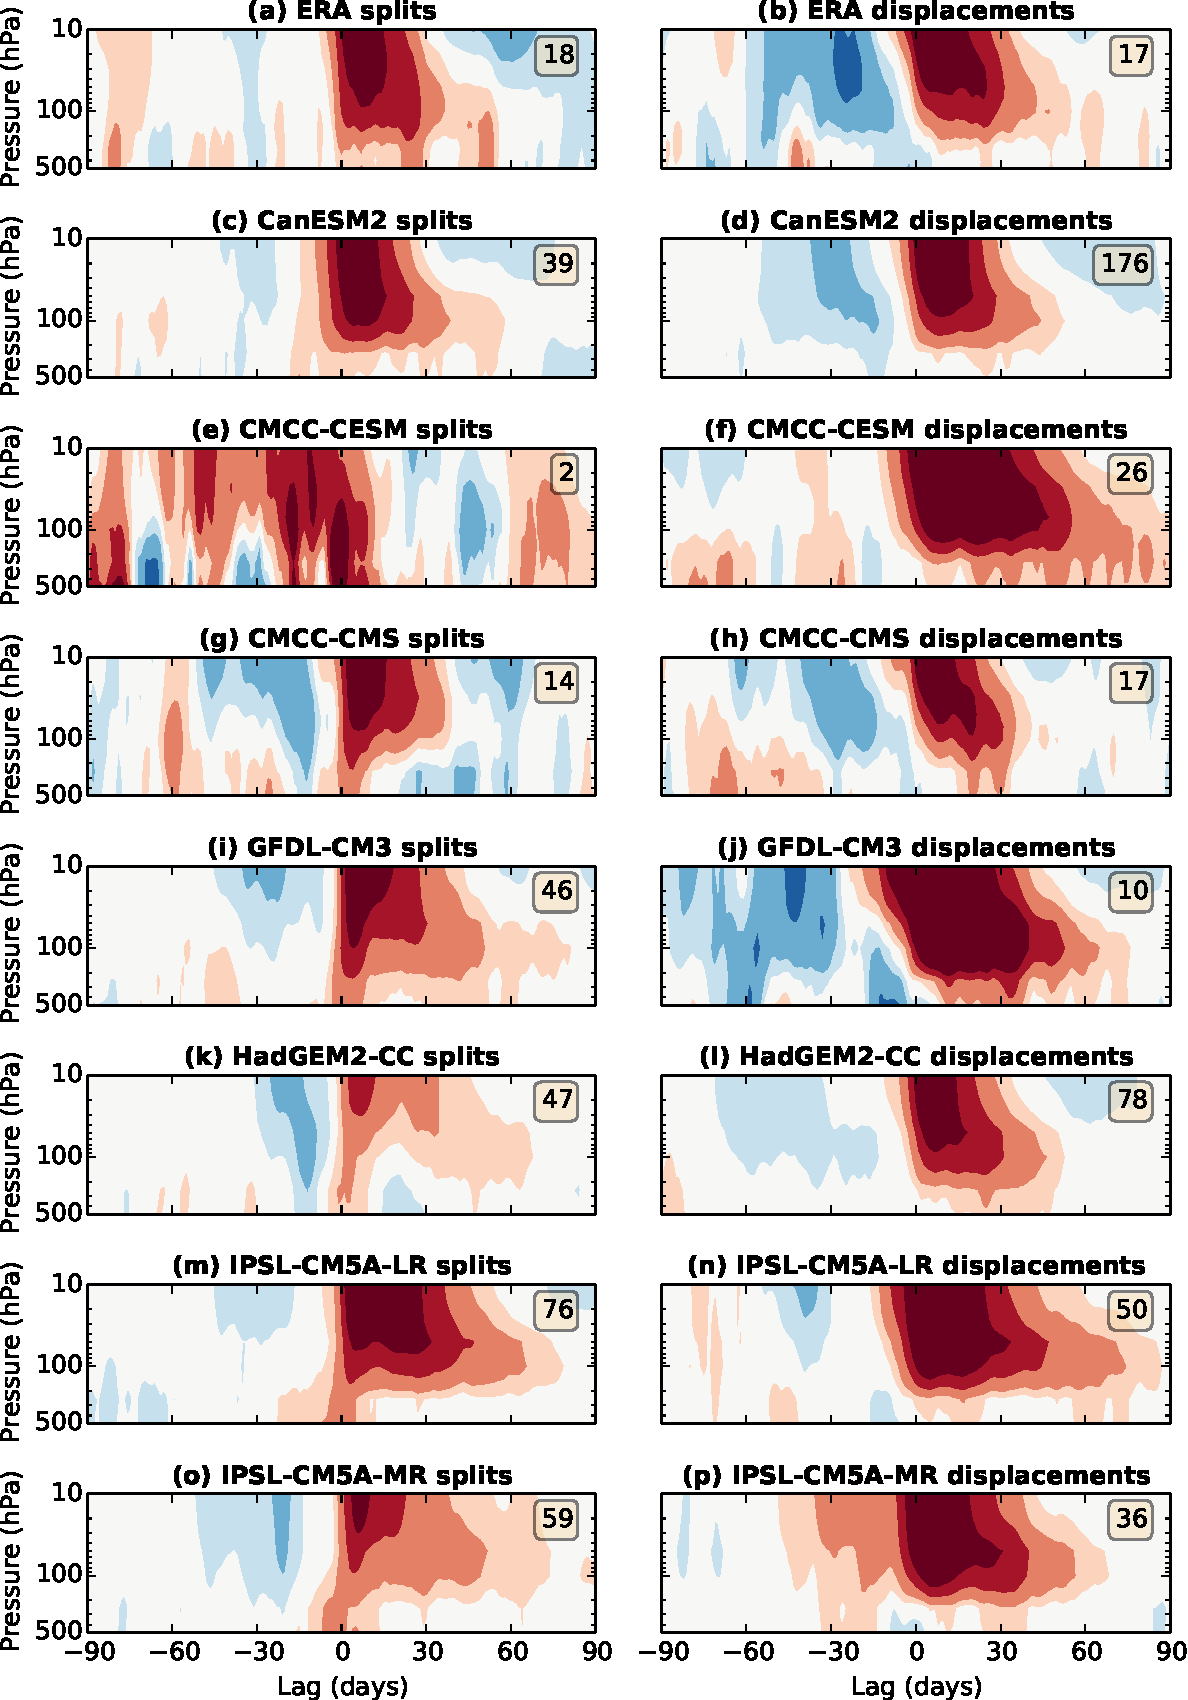
\includegraphics[width=\textwidth]{figures/chapter-models/dripping_paint1.pdf}
 \caption[NAM composites for splits and displacements in the CMIP5
 models]{Composites of normalised polar cap averaged $Z$ anomalies following
   split and displaced vortex events in ERA (a,b), the CMIP5 models, and the
   multi-model mean (C,D). Numbers in the upper right of each plot represent the
   number of events entering the composite.}
 \label{Fig2}
\end{figure}

\begin{figure}
 \ContinuedFloat
 \centering
 \noindent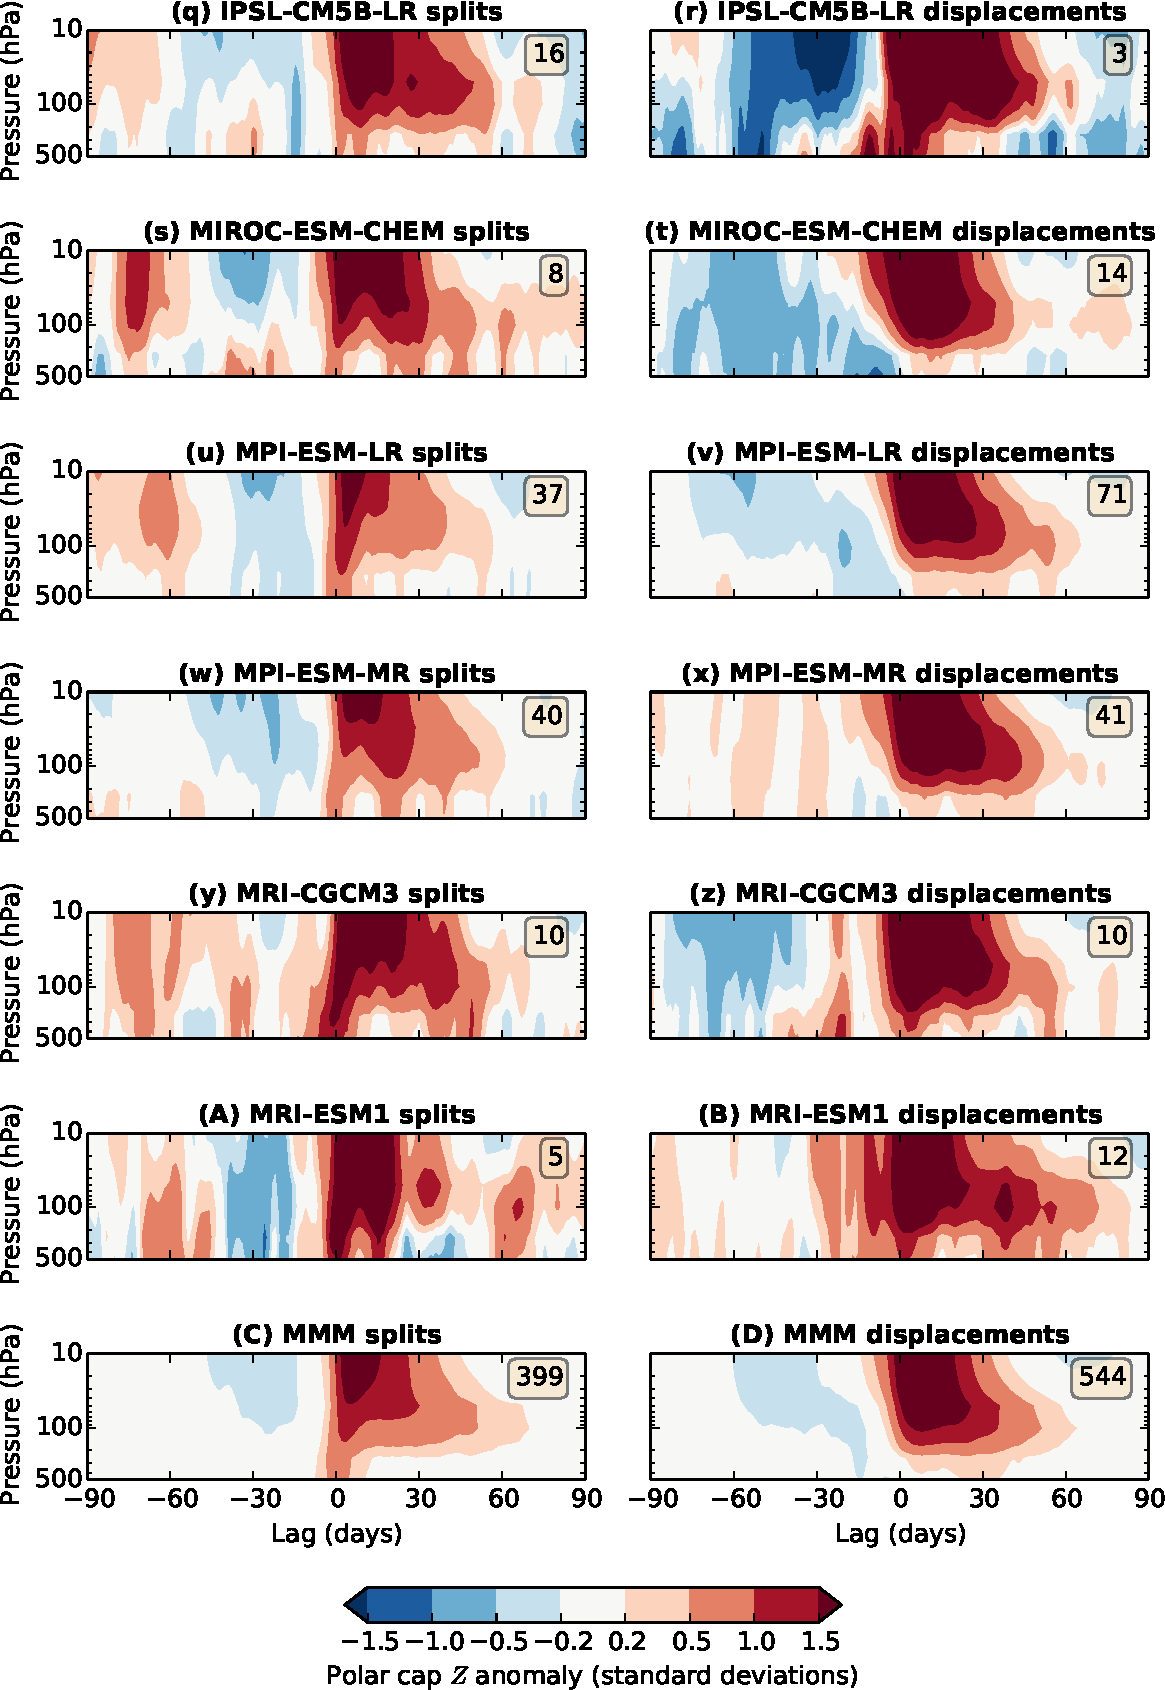
\includegraphics[width=\textwidth]{figures/chapter-models/dripping_paint2.pdf}
 \caption[]{(Continued)}
 \label{Fig2}
\end{figure}

\begin{figure}
 \centering
 \noindent\includegraphics[width=\textwidth]{figures/chapter-models/mslp_composites.pdf}
 \caption[MSLP composites following splits and displacements in the CMIP5
 models]{Composites of mean sea-level pressure averaged 0-30 days following
   split (S) and displaced (D) vortex events in the CMIP5 ensemble. Also shown
   are the ERA composite (a,b) and the multi-model mean (C,D). The multi-model
   mean is calculated as to give each event an equal weighting.}
 \label{Fig2}
\end{figure}

\begin{figure}
 \centering
 \noindent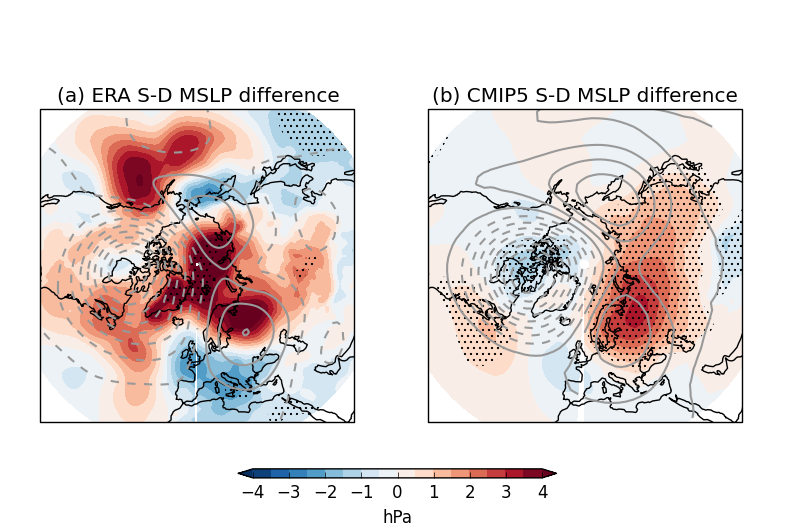
\includegraphics[width=\textwidth]{figures/chapter-models/mslp_diff.png}
 \caption[Difference of MSLP following split and displaced vortex
 events.]{Difference (S-D) of composites of mean sea-level pressure averaged 0-30 days
   following split (S) and displaced (D) vortex events in ERA and the CMIP5
   ensemble. Stippling indicates regions that are $>$95\% significant according
   to a two-tailed bootstrap test.}
 \label{Fig2}
\end{figure}


\section{Discussion}

\begin{figure}
 \centering
 \noindent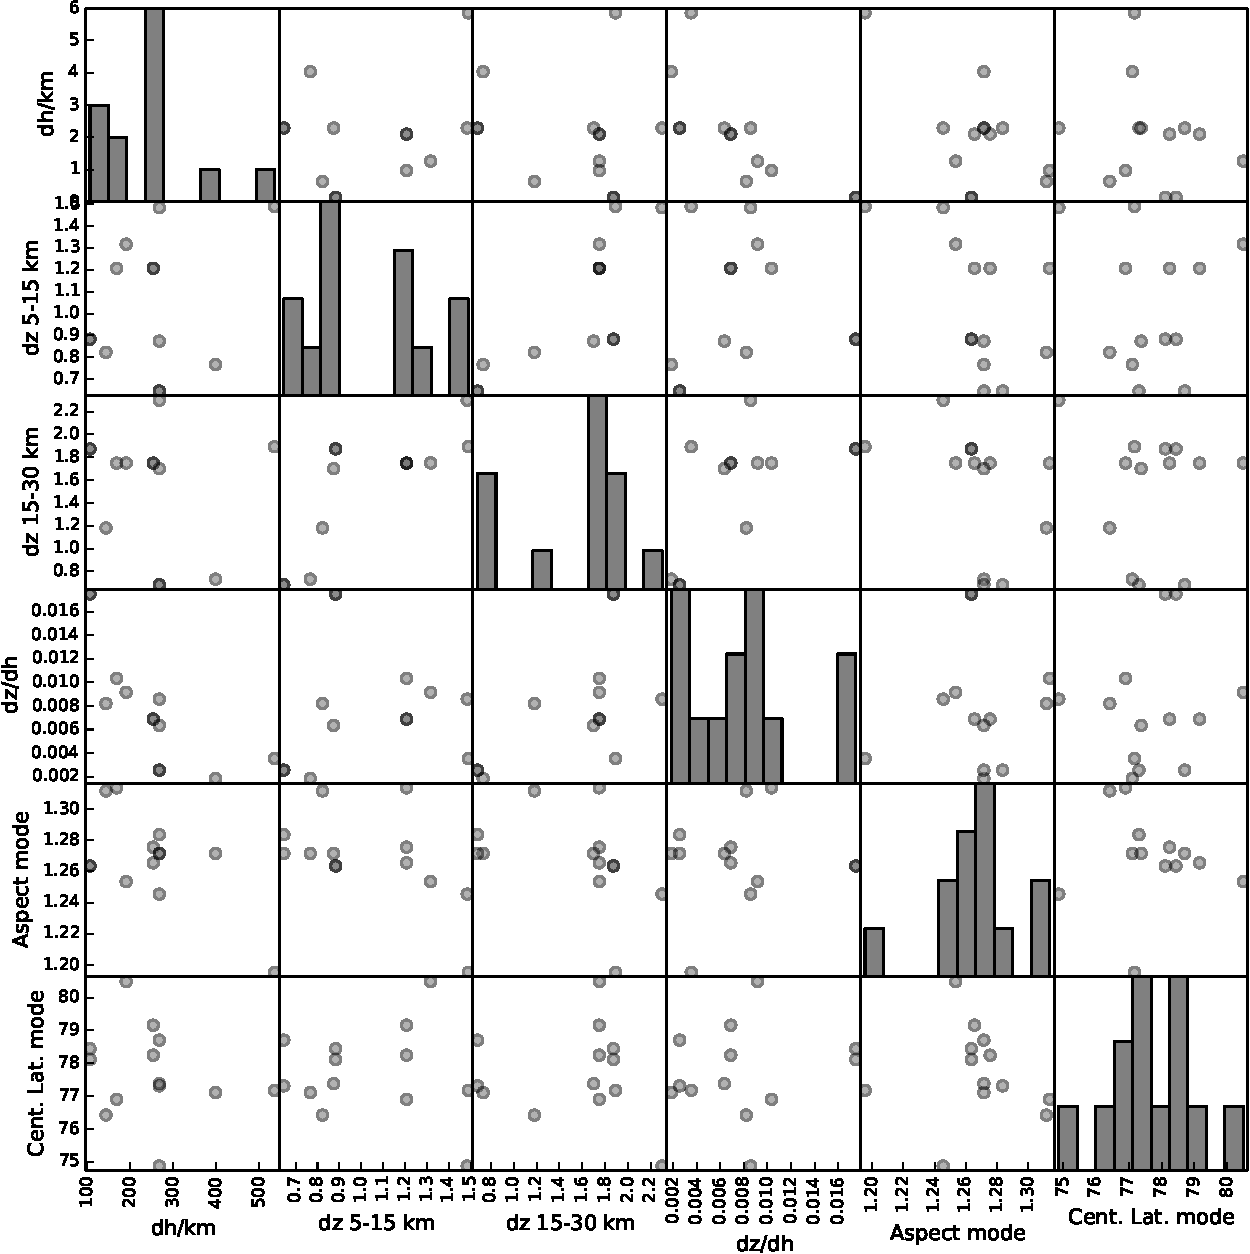
\includegraphics[width=\textwidth]{figures/chapter-models/scatter_matrix.pdf}
 \caption[Relationship between model resolution and split and displaced vortex
 events in the CMIP5 models.]{Relationship between model resolution and
   representation of split and displaced vortex events in the CMIP5
   models. Model resolution is shown as horizontal resolution ($\mathrm{d}h$),
   vertical resolution ($\mathrm{d}z$) over 5-15~km and 15-30~km, and aspect
   ratio ($\mathrm{d}z$(5-15~km)$ / \mathrm{d}h$. Also shown is the number of
   SSWs per decade, the fraction of SSWs that are splits, and the average NAM at
   500~hPa 0-30 days following SSWs. Histograms for the relevant quantities
   are shown along the leading diagonal.}
 \label{Fig2}
\end{figure}

\section{Conclusions}

%%% Local Variables:
%%% mode: latex
%%% TeX-master: "thesis"
%%% End:
